% MNS project 2010 slides
% 
% Luís Francisco Seoane Iglesias
% Mirko Dietrich - mirko.dietrich -AT- bccn-berlin -DOT- de
% 

\documentclass{beamer}
	\usepackage{color}
	
	\usepackage{beamerthemesplit}
		\usetheme{Berlin}

\title{Spike-timing-dependent plasticity}
\author{Lu\'{i}s Francisco Seoane Iglesias \& Mirko Dietrich}
\date{\today}

\logo{
\includegraphics[scale=0.2]{graphics/bccn_logo_berlin}}

\begin{document}

\frame{\titlepage}

\AtBeginSection
{
   \begin{frame}
       \frametitle{Outline}
       \tableofcontents[currentsection]
   \end{frame}
}

\section*{Outline}
\frame{
  \tableofcontents
}

\section{Hebbian Learning}
	
	\begin{frame} 
		\frametitle{Implementing Hebbian Learning}
		\begin{itemize} 
			\item Based upon \alert{integrate-and-fire} neuron model. 
					\begin{eqnarray}
						\tau_{m} \frac{dV}{dt} &=& V_{rest} - V + \textcolor{red}{g_{ex}(t)}(E_{ex} - V) + \textcolor{blue}{g_{in}(t)}(E_{in} - V)\nonumber 
					\end{eqnarray}
			\item Spikes of presynaptic neurons: 
					\begin{eqnarray}
						\alert{g_{ex}(t)} &\rightarrow& g_{ex}(t) + \bar{g}_a(t). \nonumber \\
						\textcolor{red}{g_{in}(t)} &\rightarrow& g_{in}(t) + \bar{g}_{in}. \nonumber 
					\end{eqnarray}
		\end{itemize}
	\end{frame}
	
	\begin{frame} 
		\frametitle{Implementing Hebbian Learning}
		\begin{itemize} 
			\item The voltage of the post-synaptic neuron decays toward: 
				\begin{eqnarray}
					V_{rest} &-& V + \textcolor{red}{g_{ex}(t)}(E_{ex} - V) + \textcolor{blue}{g_{in}(t)}(E_{in} - V). \nonumber \\
					\tau_m &=& 20 ms. \nonumber
				\end{eqnarray}
			\item The connectivities $g_{ex}(t)$ and $g_{in}(t)$ decay toward zero: 
				\begin{eqnarray} 
					\tau_{ex} &=& 5ms. \nonumber \\
					\tau_{in} &=& 5ms. \nonumber
				\end{eqnarray}
		\end{itemize}
	\end{frame}

	\begin{frame} 
		\frametitle{Implementing Hebbian Learning}
		\begin{columns} 
			\column{0.5\textwidth} 
				\begin{figure} 
					\centering
					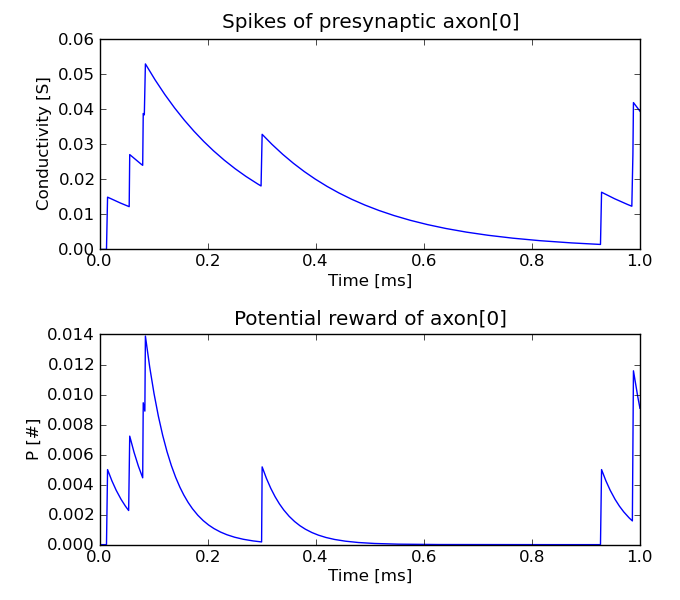
\includegraphics[width=\textwidth]{graphics/demo/fig01} 
				\end{figure} 
			\column{0.5\textwidth} 
				\begin{block}{$g_{ex}(t) \rightarrow g_{ex}(t) + \alert{\bar{g}_a(t)}$}
					\hspace{5 mm}
					\begin{itemize} 
						\item Axons spike with a certain frequency. \\
						\hspace{5 mm}
						\item When spike, a \alert{potential \emph{reward} $P(t)$} accumulates. 
					\end{itemize}
				\end{block}
		\end{columns}
	\end{frame}
	
	\begin{frame} 
		\frametitle{Implementing Hebbian Learning}
		\begin{columns} 
			\column{0.5\textwidth} 
				\begin{figure} 
					\centering
					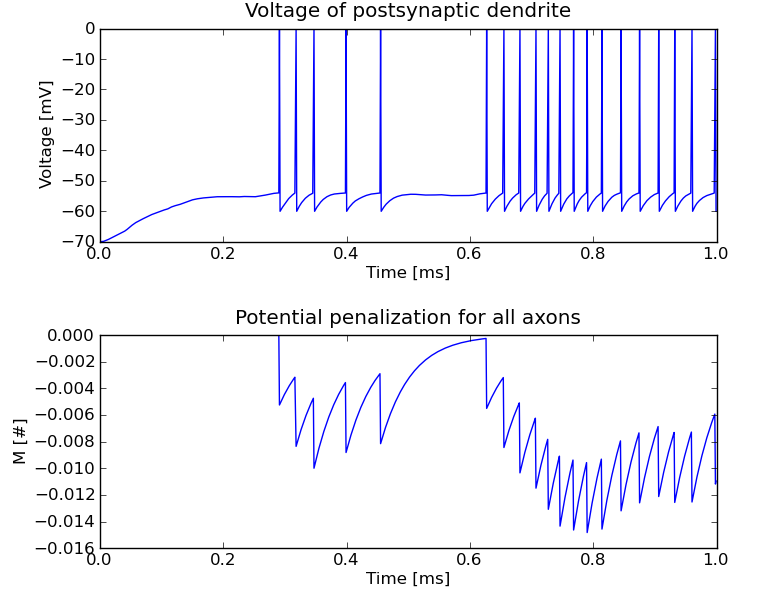
\includegraphics[width=\textwidth]{graphics/demo/fig02} 
				\end{figure} 
			\column{0.5\textwidth} 
				\begin{block}{$g_{ex}(t) \rightarrow g_{ex}(t) + \alert{\bar{g}_a(t)}$}
					\hspace{5 mm}
					\begin{itemize} 
						\item The dendrite spikes induced by the axons. \\
						\hspace{5 mm}
						\item A \alert{\emph{penalty} function $M(t)$} also accumulates, elicited by the spike of the dentrite. 
					\end{itemize}
				\end{block}
		\end{columns}
	\end{frame}
	
	\begin{frame} 
		\frametitle{Implementing Hebbian Learning}
		\begin{itemize} 
			\item Both reward $P(t)$ and penalty $M(t)$ decay toward zero with: 
				\begin{eqnarray} 
					\tau_M = 20 ms \nonumber \\
					\tau_P = 20 ms \nonumber
				\end{eqnarray}
			\item Time of decay should be larger than the decay of $g_{ex}(t)$ and $g_{in}(t)$. 
		\end{itemize}
	\end{frame}
	
	\begin{frame} 
		\frametitle{THE \alert{BUG}} 
		\begin{columns} 
			\column{0.5\textwidth} 
				\begin{figure} 
					\centering
					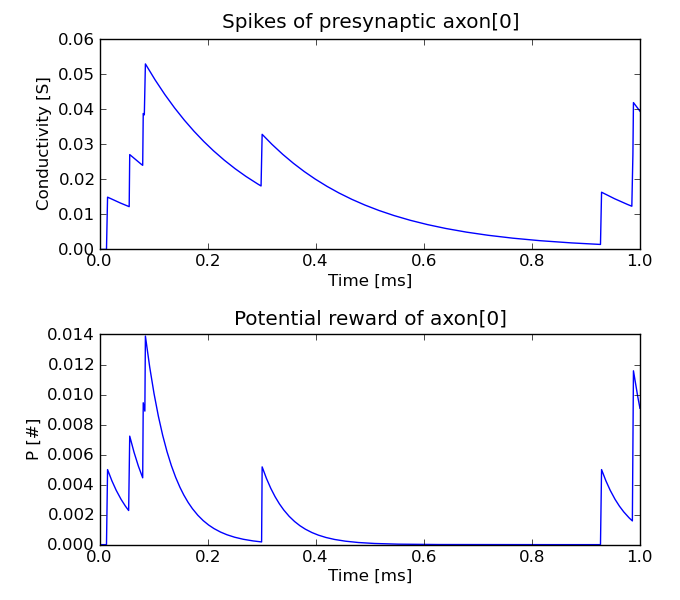
\includegraphics[width=\textwidth]{graphics/demo/fig01} 
				\end{figure} 
			\column{0.5\textwidth} 
				\begin{block}{THE \alert{BUG}}
					\vspace{5 mm}
					def exponentialDecay(x,param):
					\hspace*{4mm}tau $=$ param[0]\\
					\hspace*{4mm}resting\_value $=$ param[1]
					\hspace*{4mm}\alert{return $-(x-$resting\_value)*tau}
					\hspace*{4mm}return $-(x-$resting\_value)/tau
				\end{block}
		\end{columns}
	\end{frame}
	
	\begin{frame} 
		\frametitle{THE \alert{BUG}} 
		\begin{block}{THE \alert{BUG}}
			\begin{itemize} 
				\item \alert{EigenTime} shows up to be \alert{critical}: 
				\begin{itemize} 
					\item Wrong parameters lead to exceptionally wrong results. 
					\item Decay of functions $P(t)$ and $M(t)$ \alert{has to be slower} than the decay of $g_{ex}(t)$ and $V(t)$. 
					\item Thus: the \alert{$\tau$} ruling the decay \alert{must be larger} for $M(t)$ and $P(t)$. 
				\end{itemize}
			\end{itemize}
		\end{block}
	\end{frame}
	
\section{Balanced Excitation}

	\begin{frame} 
		\frametitle{Setup} 
		\begin{itemize} 	
			\item 200 inhibitory presynaptic neurons. 
			\begin{itemize} 
				\item Firing rate: $10 Hz$. \\
				\hspace{5 mm}
			\end{itemize}
			\item $1000$ excitatory presynaptic neurons. 
			\begin{itemize} 
				\item Firing rate $\in [10,40]Hz$. 
			\end{itemize}
		\end{itemize} 
	\end{frame} 
	\begin{frame}
		\frametitle{Setup} 
		\begin{itemize}
			\item Hebbian Learning algorithm runs until $g_a(t)$ remains steady. 
			\begin{itemize}
				\item We want to study this distribution for different firing rates of the excitatory neurons. \\
				\hspace{5 mm}
				\item Once a steady distribution is reached: 
				\begin{itemize} 
					\item Study of the induced firing rate in the post-synaptic neuron. 
					\item Study of the variance of the interval between spikes in the post-synaptic neuron. 
				\end{itemize}
			\end{itemize}
		\end{itemize}
	\end{frame}

\end{document}


















 